\documentclass[10pt,a4paper]{article}
\usepackage[utf8]{inputenc}
\usepackage{amsmath}
\usepackage{amsfonts}
\usepackage{amssymb}
\usepackage{makeidx}
\usepackage{graphicx}
\usepackage{tikz}
\usetikzlibrary{calc,shapes.geometric, arrows}
\author{Xuanyu Wang}
\begin{document}
	\begin{figure}[hp]
		\centering
		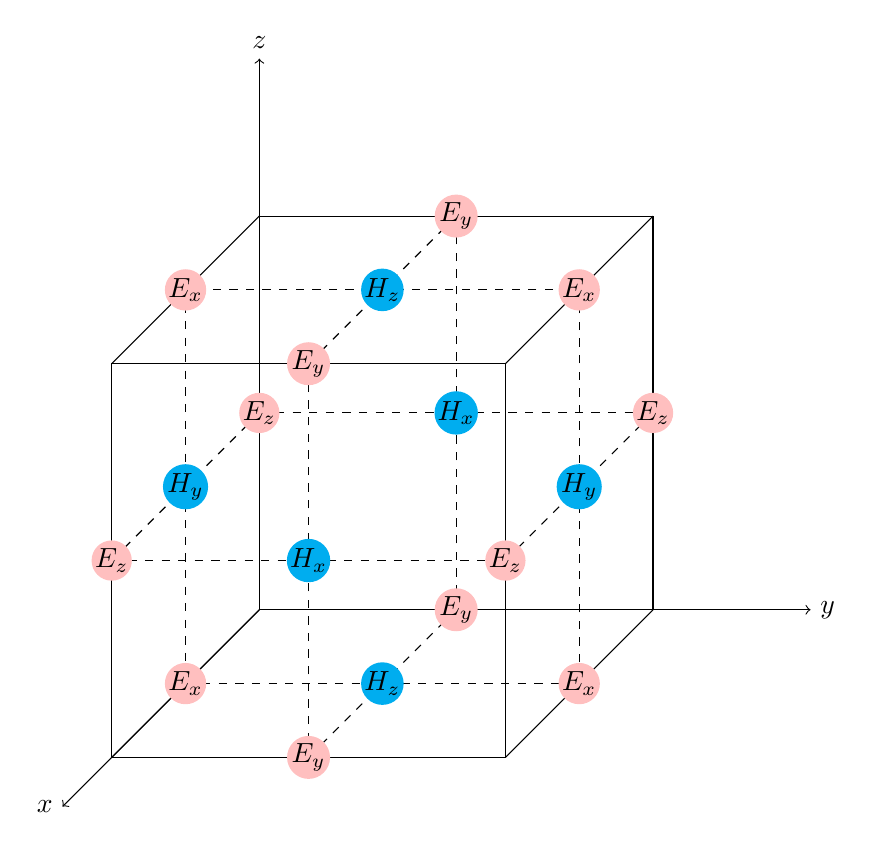
\begin{tikzpicture}
		\def \len {5}
		\def \hlen {2.5}
		\def \coe {-0.75}
		
		%back rectangle wigh dashline
		\draw(0,0) rectangle +(\len,\len);
		\draw [dashed] ($(0,0)+0.5*(0,\len)$) -- +(\len,0);
		\draw [dashed] ($(0,0)+0.5*(\len,0)$) -- +(0,\len);
		
		%front rectangle wigh dashline
		\draw($(0,0)+\coe*(\hlen,\hlen)$) rectangle +(\len,\len);
		\draw [dashed] ($(0,0)+(0,\hlen)+\coe*(\hlen,\hlen)$) -- +(\len,0);
		\draw [dashed] ($(0,0)+(\hlen,0)+\coe*(\hlen,\hlen)$) -- +(0,\len);
		
		%connect two rectangle
		\draw (0,0) -- ($(0,0)+\coe*(\hlen,\hlen)$);
		\draw ($(0,0)+(0,\len)$) -- ($(0,0)+(0,\len)+\coe*(\hlen,\hlen)$);
		\draw ($(0,0)+(\len,0)$) -- ($(0,0)+(\len,0)+\coe*(\hlen,\hlen)$);
		\draw ($(0,0)+(\len,\len)$) -- ($(0,0)+(\len,\len)+\coe*(\hlen,\hlen)$);
		
		%all dashline
		\draw [dashed] ($(0,0)+(0,\hlen)$) -- ($(0,0)+(0,\hlen)+\coe*(\hlen,\hlen)$);
		\draw [dashed] ($(0,0)+(\hlen,0)$) -- ($(0,0)+(\hlen,0)+\coe*(\hlen,\hlen)$);
		\draw [dashed] ($(0,0)+(\len,\hlen)$) -- ($(0,0)+(\len,\hlen)+\coe*(\hlen,\hlen)$);
		\draw [dashed] ($(0,0)+(\hlen,\len)$) -- ($(0,0)+(\hlen,\len)+\coe*(\hlen,\hlen)$);
		
		\draw [dashed] ($(0,0)+0.5*\coe*(\hlen,\hlen)$) -- ++(\len,0) -- ++(0,\len) -- ++(-\len,0) -- cycle;
		
		%axis
		\draw [->] (0,0) -- +(\len+2,0) node[right]{$y$};
		\draw [->] (0,0) -- +(0,\len+2) node[above]{$z$};
		\draw [->] (0,0) -- +($(0,0)-(\hlen,\hlen)$) node[below,left]{$x$};
		
		%nodes
		%Hx
		\node[shape=circle,fill=cyan,inner sep=0pt] at (\hlen,\hlen) {$H_x$};
		\node[shape=circle,fill=cyan,inner sep=0pt] at ($(\hlen,\hlen)+\coe*(\hlen,\hlen)$) {$H_x$};
		%Hz		
		\node[shape=circle,fill=cyan,inner sep=0pt] at ($(0,0)+(\hlen,0)+0.5*\coe*(\hlen,\hlen)$) {$H_z$};
		\node[shape=circle,fill=cyan,inner sep=0pt] at ($(0,0)+(\hlen,0)+0.5*\coe*(\hlen,\hlen)+(0,\len)$) {$H_z$};
		%Hy
		\node[shape=circle,fill=cyan,inner sep=0pt] at ($(0,0)+(0,\hlen)+0.5*\coe*(\hlen,\hlen)$) {$H_y$};
		\node[shape=circle,fill=cyan,inner sep=0pt] at ($(0,0)+(0,\hlen)+0.5*\coe*(\hlen,\hlen)+(\len,0)$) {$H_y$};
		%Ez
		\node[shape=circle,fill=pink,inner sep=0pt] at ($(0,\hlen)$) {$E_z$};
		\node[shape=circle,fill=pink,inner sep=0pt] at ($(0,\hlen)+\coe*(\hlen,\hlen)$) {$E_z$};
		\node[shape=circle,fill=pink,inner sep=0pt] at ($(0,\hlen)+(\len,0)$) {$E_z$};
		\node[shape=circle,fill=pink,inner sep=0pt] at ($(0,\hlen)+\coe*(\hlen,\hlen)+(\len,0)$) {$E_z$};
		%Ex
		\node[shape=circle,fill=pink,inner sep=0pt] at ($(0,\hlen)+0.5*\coe*(\hlen,\hlen)+(0,\hlen)$) {$E_x$};
		\node[shape=circle,fill=pink,inner sep=0pt] at ($(0,\hlen)+0.5*\coe*(\hlen,\hlen)+(\len,0)+(0,\hlen)$) {$E_x$};
		\node[shape=circle,fill=pink,inner sep=0pt] at ($(0,\hlen)+0.5*\coe*(\hlen,\hlen)+(0,-\hlen)$) {$E_x$};
		\node[shape=circle,fill=pink,inner sep=0pt] at ($(0,\hlen)+0.5*\coe*(\hlen,\hlen)+(\len,0)+(0,-\hlen)$) {$E_x$};
		%Ey
		\node[shape=circle,fill=pink,inner sep=0pt] at ($(\hlen,\hlen)+(0,\hlen)$) {$E_y$};
		\node[shape=circle,fill=pink,inner sep=0pt] at ($(\hlen,\hlen)+\coe*(\hlen,\hlen)+(0,\hlen)$) {$E_y$};
		\node[shape=circle,fill=pink,inner sep=0pt] at ($(\hlen,\hlen)+(0,-\hlen)$) {$E_y$};
		\node[shape=circle,fill=pink,inner sep=0pt] at ($(\hlen,\hlen)+\coe*(\hlen,\hlen)+(0,-\hlen)$) {$E_y$};
		\end{tikzpicture}
		%\caption{The spatial discrete structure of Yee cell}\label{ch2 fig: yee cell}
	\end{figure}
\end{document}